% multiple1902 <multiple1902@gmail.com>
% intro.tex
% Copyright 2011~2012, multiple1902 (Weisi Dai)
% https://code.google.com/p/xjtuthesis/
%
% It is strongly recommended that you read documentations located at
%   http://code.google.com/p/xjtuthesis/wiki/Landing?tm=6
% in advance of your compilation if you have not read them before.
%
% This work may be distributed and/or modified under the
% conditions of the LaTeX Project Public License, either version 1.3
% of this license or (at your option) any later version.
% The latest version of this license is in
%   http://www.latex-project.org/lppl.txt
% and version 1.3 or later is part of all distributions of LaTeX
% version 2005/12/01 or later.
%
% This work has the LPPL maintenance status `maintained'.
%
% The Current Maintainer of this work is Weisi Dai.
%

\chapter{论文相关理论与技术}
\echapter{Relative Theory and Technology}

    文字检测按照其研究目标和存储介质的不同,可分为数字图像文字检测、视频图像中的文字检测和自然场景图像中的文字检测。其中,由于自然场景中的文字会遭受背景复杂多样性,以及图像质量易被光照、阴影、遮挡等环境因素影响,致使自然场景图像的文字检测相比于其它图像对检测算法的健壮性要求更高。这些年来,学者们在文字检测领域进行了大量的研究和实验工作,提出了许多不同的方法,检测效果也在逐年提升。但是在ICDAR等公开数据集上的测试结果表明,目前的这些自然场景图像中的文字检测结果仍有提高空间,所以仍是文字检测领域内的一个热点方向。场景图像文字检测方法根据流程不同,可分为基于区域的文字检测方法和基于连通部件的文字检测方法两大类。下面整理并分别介绍近年来这两类文字检测的相关方法。

    \section{基于区域的场景文字检测方法}
    \esection{Region-based Method}

    基于区域的文字检测方法,是基于文子有别于背景的视觉特征来区分文字区域与背景区域的。使用较多的视觉特征主要包括纹理、边缘及颜色等。因为每个文字都是用来传递信息的特定符号,其纹理与一般背景并不相同,同时文字相比于背景也有着更强的对比度和显著的颜色,所以包含着文字的那些区域和背景图像区域有着不同的视觉特征,因而可以用来区分文字区域与非文字区域。

    大部分基于区域的方法一般都会利用滑动窗来获取候选的包含文字的局部图像区域,因此在有些方法中也称其为基于滑动窗的文字检测算法。如图\ref{fig.c2_region_based} 所示,这是1个典型的基于区域的文字检测方法的流程示例。在该流程示例中,首先利用滑动窗来得到局部图像区域以作为候选区域,然后提取区域中的颜色、纹理等视觉特征,最后结合分类器以进行文字与非文字区域的分类判别,输出结果是检测出来的文字区域。

    \begin{figure}[!h]
    \centering
    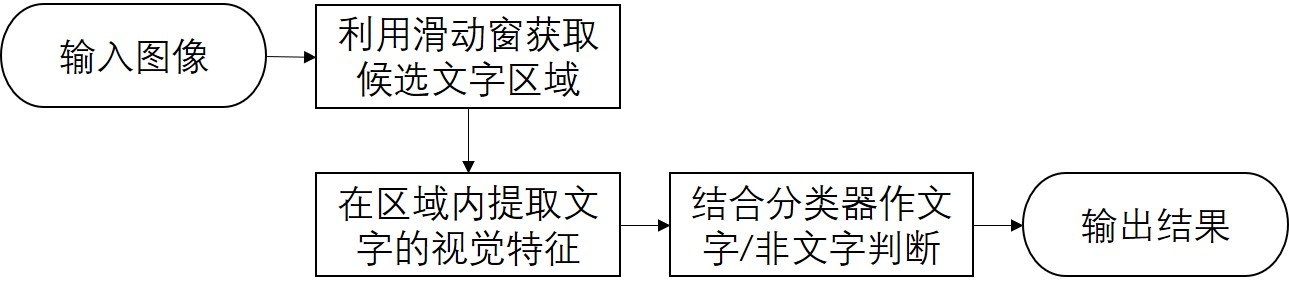
\includegraphics[width=\textwidth]{c2_region_based.jpg}
    \caption{基于区域的文字检测方法的流程示例}
    \label{fig.c2_region_based}
    \end{figure}

    Chen等\cite{Chen2004Detecting}利用滑动窗扫描得到文字区域并获取区域中的79个特征,然后构造4个级联的Adaboost 分类器来分类和筛选这些候选文字区域,最后用OCR软件识别图像中文字信息。其中4个级联的分类器是由不同的文字底层特征构造而成的弱分类器,通过利用Adaboost方法将这些弱分类器组合学习而获得1 个分类文字与背景的强分类器。用于训练弱分类器的三组特征分别是:候选区域内竖直和水平方向灰度的标准差与平均值;区域内的统计梯度信息;区域内边缘组合特征。而本方法中使用的79个特征,分散在4层的级联分类器中,分别有1、10、30和50维文字特征。最后OCR使用的技术是用Niblack方法来二值化检测到的文字区域以识别出图像中的文字。

    Pan等\cite{Pan2011A}设计了一种基于滑动窗的文本区域的检测器,用于估算图像金字塔中的文本行存在的置信度和尺度信息,在每个尺度中使用滑动窗扩得到候选文字区域并利用WaldBoost分了器对各个窗口的文字置信度进行预测。然后该文利用基于连通部件类别中的局部二值化方法对候选文本分量进行分割。为有效的过滤掉非文本的部件,这篇文章提出了一个考虑一元组件的属性和二元上下文的成分关系的条件随机场(CRF)模型。其中,一元特征表征单个部件自身的文字置信度,例如有占空比、紧密度、轮廓梯度以及宽高比等;而二元特征表征相邻候选文字连通部件即上下文的关系,如颜色、形状、尺度和距离等差异。最后基于能量最小化方法将这些文本组件分类到文本行中。

    上述文字检测方法一般使用人工设计的特征,例如颜色、纹理、笔画宽度等,进行文字与非文字分类。虽然这些特征可以区分大多数的文字与非文字,部分与文字相似的背景却难以区分,例如窗户、砖块等。为了能够更好地反映文字的属性,近年来许多方法开始采用深度学习技术,其中最常用的一种结构是卷积神经网络(CNN)。CNN是一种特殊的前馈人工神经网络,其中的神经元之间的连接关系类似于视觉皮层的结构。同时,因为CNN能够利用图像中的局部空间相关性,故CNN特别适合于处理计算机视觉问题,尤其是目标识别领域,例如在手写字符识别、交通标志识别、图像分类等方面都取得了优秀的表现。

    \begin{figure}[!h]
    \centering
    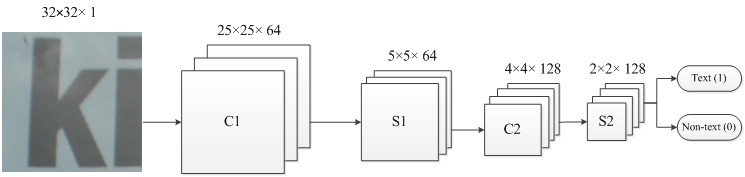
\includegraphics[width=\textwidth]{c2_wangtao_cnn.jpg}
    \caption{Wang等\cite{Wang2012End}采用的CNN网络框架}
    \label{fig.c2_wangtao_cnn}
    \end{figure}

    Wang等\cite{Wang2012End}设计的端对端文字检测和识别框架的核心即是卷积神经网络CNN。该方法首先利用滑动窗在图像金字塔上扫描得到候选文字图像块区域,然后将这些图像块区域缩放成$32\times32$像素大小的正方形小图块。接着这些图块的灰度图会输入到1个训练好的,含有2层卷积的CNN网络中进行特征的提取,以及对这些图块区域的分类。其中,卷积神经网络CNN的结构如图\ref{fig.c2_wangtao_cnn}所示:输入图像小块经过第1层的64个卷积模板的卷积操作后,得到64个$25\times25$的响应图,紧接着再执行平均池化获得相应的$5\times5$ 的响应;然后再通过第2卷积层中的128个卷积模板的卷积操作及后续的平均池化操作后,得到$2\times2\times128$的全连接层。在通过上CNN 网络的特征提取和分类后,最后再利用非极大抑制NMS操作来筛选重叠的分类结果以获得文字行定位结果。此外还构建62类的分类器来识别图块中的文字。

    \begin{figure*}[!h]
    \centering
    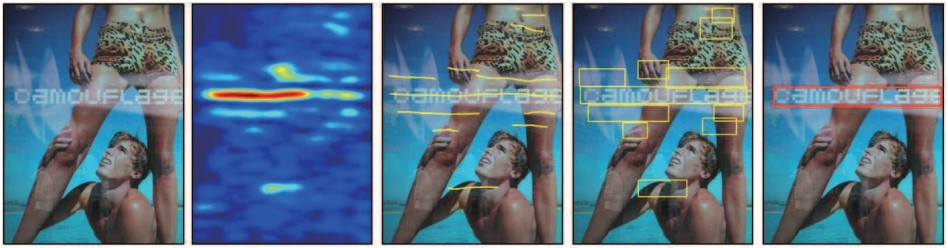
\includegraphics[width=\textwidth]{./figures/c2_zhang_cnn.jpg}
    \begin{minipage}[t]{0.18\linewidth}
    \centerline{ \small (a) 输入原图}
    \end{minipage}
    \begin{minipage}[t]{0.18\linewidth}
    \centerline{ \small (b) 概率图}
    \end{minipage}
    \begin{minipage}[t]{0.18\linewidth}
    \centerline{ \small (c) 对称轴}
    \end{minipage}
    \begin{minipage}[t]{0.18\linewidth}
    \centerline{ \small (d) 候选文本行}
    \end{minipage}
    \begin{minipage}[t]{0.18\linewidth}
    \centerline{ \small (d) CNN分类结果}
    \end{minipage}
    \caption{基于对称性文本行检测算法流程}
    \label{fig.c2_zhang_cnn}
    \end{figure*}

    Zhang等\cite{Zhang2015Symmetry}提出一种利用滑动窗提取对称性特征的文字检测算法。该方法首先设计1个对称性计算模板来计算滑动窗口内区域的梯度直方图、局部二值模式LBP以及颜色等特征的相似度,然后将这些特征输入随机森林分类器从而得到每个像素属于文本行对称轴的概率图。接着把概率图上概率相近的像素集中形成文本行对称轴并用CRF进行更准确的分类。然后在此基础上利用窗口尺寸生成候选文本行并作多个尺度上的文本行的投影融合。最后采用训练好的CNN分类器去掉非文字的图像区域。从这个方法的实验结果来看,利用深度学习来分类候选文本行区域,可将其中真实的文字部分精准的辨别出来,因而能较大程度的提高文本检测的成绩。

    \begin{table*}[!h]
    \centering
    \caption{基于区域的相关文字检测方法}
    \begin{tabular}{p{0.17\textwidth}|p{0.1\textwidth}| p{0.63\textwidth}}
    \hline
    作者 & 年份 & 方法概述 \\
    \hline
    Chen等\cite{Chen2004Detecting} & 2004年 & 区域特征,滑动窗检测,以及SVM分类器;\\
    Pan等\cite{Pan2011A} & 2011年 &   条件随机场,滑动窗检测,以及waldBoost分类器\\
    Wang等\cite{Wang2012End} & 2012年 & 卷积神经网络和滑动窗检测 \\
    Zhang等\cite{Zhang2015Symmetry} & 2015年 & 对称性特征,滑动窗检测以及卷积神经网络 \\
    \hline
    \end{tabular}
    \label{tab.c2_region_based}
    \end{table*}

    表格\ref{tab.c2_region_based}总结了基于区域的相关文字检测方法。(优缺点;wang的方法的问题:第3章的问题提出;zhang的方法中怎么利用CNN,对我的方法的启发)

    \section{基于连通部件的场景文字检测方法}
    \esection{Connected Component-based Method}

    基于连通部件的检测方法,将文字看做是一些连通部件的集合,所以这类方法是把连通部件作为处理对象的文字检测算法。这种基于连通部件来检测场景图像中文字的原理是:因为文字之间的笔画、纹理、对比度以及颜色等特征具有一致性,所以可通过笔画宽度转换、图像分割或最稳定极值区域提取等处理,来把候选文字的像素组成一系列的连通部件。
    
    如图\ref{fig.c2_cca_based}所示,这是一个典型的基于连通部件的检测方法的流程示例。在此类方法的流程中,通常首先会标记可能同属一个字符连通部件的像素,然后在分割连通部件的阶段通过把文字从背景中分离出来而得到候选的文字部件;接着在分析连通部件的阶段,首先提取笔画、几何、边缘及颜色等这些基于连通部件的特征,然后利用分类器来过滤掉非文字的部件;最后留下来的文字检测结果作为输出。

    \begin{figure}[!h]
    \centering
    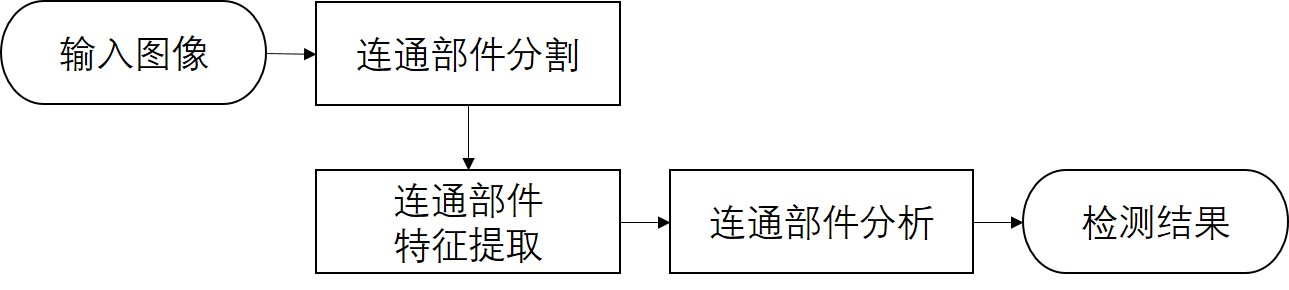
\includegraphics[width=\textwidth]{c2_cca_based.jpg}
    \caption{基于连通部件的文字检测方法的流程示例}
    \label{fig.c2_cca_based}
    \end{figure}
    
    Epshetein等\cite{Epshtein2010Detecting}提出用笔画宽度变换方法SWT来检测文字,促进了基于边缘(是连通部件中的一种)的文字检测算法的研究。这个方法根据图像里的文字笔画的宽度通常较为均一的属性,来过滤掉非文字边缘的像素。该方法首先利用Canny算子在场景文字图像的灰度图上求取图像中各目标的边缘,然后执行笔画宽度转换算法来计算笔画宽度图,其关键思路为:以边缘上的每个像素点为起始位置,沿该起始位置的梯度正负方向出发进行搜索,以找到梯度方向与起始位置点的方向近似相反的另一个边缘点,那么标记两像素点间的距离即为这个边缘的笔画宽度。在笔画宽度转换之后,再利用连通部件方法聚合起具有相近笔画宽度的像素点,以生成候选文字区域并方便后续的连通部件分析。最后使用启发性规则,例如欧拉数、宽高比等特征来过滤以得到真实文字区域。

    \begin{table*}[!h]
    \centering
    \caption{基于连通部件的相关文字检测方法}
    \begin{tabular}{p{0.17\textwidth}|p{0.1\textwidth}| p{0.63\textwidth}}
    \hline
    作者 & 年份 & 方法概述 \\
    \hline
    Epshetein等\cite{Epshtein2010Detecting} & 2010年 & 候选文字筛选,笔画宽度转换SWT,文本行生成;\\
    Neumann等\cite{Neumann2011Text} & 2011年 &   最稳定极值区域MSER,穷举搜索\\
    Dollar等\cite{Dollar2015Fast} & 2015年 & 结构化边缘检测子,随机森林分类器 \\
    Yu等\cite{Yu2016Scene} & 2016年 & 文字的特征池,文字的边缘重组,以及SVM分类器 \\
    \hline
    \end{tabular}
    \label{tab.c2_connected_component_based}
    \end{table*}

    \section{本章小结}
    \esection{Brief Summary}

